\documentclass{article}
\usepackage{graphicx}
\usepackage{xcolor}
\usepackage{pgfplots}
\usepackage{fancyvrb}
\usepackage{hyperref} 


\begin{document}

\begin{titlepage}
    \centering
    {\bfseries\LARGE Universidad Internacional Menéndez Pelayo  \par}
    \vspace{1cm}
    {\scshape\Large Máster en Investigación en Inteligencia Artificial    \par}
    \vspace{3cm}
    {\scshape\Huge Planificación automática Práctica 1 \par}
    \vspace{3cm}
    {\itshape\Large \href{https://github.com/AlfonsoLozana/UIMP-PA-Practica1}{\textcolor{blue}{AlfonsoLozana/UIMP-PA-Practica1}} \par} % Cambia el color y el estilo aquí
    \vfill
    {\Large Autor: \par}
    {\Large Alfonso Lozana Cueto \par}
    \vfill
\end{titlepage}

\section{Introducción}
En esta práctica nos enfocamos en problemas PDDL, utilizando como punto de partida dos dominios predefinidos: "Robots" y "Satellite".
El objetivo principal es modificar el dominio de los Robots y generar nuevos problemas dentro de este contexto actualizado. 
Posteriormente, emplearemos el planificador Metric-FF para resolver los problemas en los tres dominios.

Este informe detalla los cambios realizados en el dominio y los problemas, así como los resultados obtenidos mediante las ejecuciones 
del planificador Metric-FF. En la última sección del documento, se analizarán los resultados obtenidos.

 \section{Cambios en el Dominio y Problema}

 \subsection{Cambios en el Dominio}
 Dado el dominio de \textit{Robots}, se pide realizar una serie de modificaciones:

 \begin{itemize}
     \item Definir dos subtipos de robots: \textit{robots-brazos} y \textit{robots-cesta}.
     \item \textit{Robots-brazos}: Pueden levantar objetos (\textit{pobject}) de sitios (\textit{location}) y dejarlos en otro lugar. Además, al no llevar una cesta, su capacidad máxima es de dos objetos, uno en cada brazo.
     \item \textit{Robots-cesta}: Carecen de brazos, por lo que no pueden levantar o dejar objetos directamente. Dependen de los \textit{robots-brazos} para introducir o quitar objetos en la cesta. Además, pueden contener un número infinito de objetos.
     \item Añadir acción adicional a los \textit{robots-brazo}: dar o tomar objetos de otros robots.
 \end{itemize}
 
 Para llevar a cabo estos cambios, siempre se tuvo en cuenta la simplificación y legibilidad del código desarrollado. Tras varias iteraciones, estos fueron los cambios realizados:
 
 \begin{enumerate}
     \item Se añadió el tipo \textit{:fluents} para controlar el número de brazos que tiene un robot de tipo robot-brazo.
     \item Se introdujeron dos nuevos tipos: \textit{robot-brazo} y \textit{robot-cesta} como subtipos de \textit{robot}.
     \item Se implementaron nuevos predicados para dar soporte a las funcionalidades añadidas. 
 
 
 \begin{itemize}
     \item \texttt{(in-cesta ?r - robot ?p - pobject)}: indica si un objeto está en una cesta.
     \item \texttt{(has-brazo ?r - robot)}: indica si un robot tiene brazos.
 \end{itemize}
 
 \item También se añadió una nueva función para indicar cuántos brazos tiene disponible un robot:
 \begin{verbatim}
     (brazos-libres ?r - robot)
 \end{verbatim}
\end{enumerate}
 En cuanto a las acciones, los cambios son los siguientes:
 
 \begin{itemize}
    \item En la acción \texttt{MOVE}, no se tuvo que realizar ninguna modificación.
    \item En la acción \texttt{PICK-UP}, se cambió el tipado de los parámetros, ya que son funciones exclusivas para \textit{robot-brazo}.
    Además, se añadió una precondición \texttt{\textgreater{ (brazos-libres ?rb) 0}} para controlar los brazos disponibles que tiene un robot, así como un efecto que ocupa un brazo \texttt{({decrease (brazos-libres ?rb) 1})}.
    
    \begin{Verbatim}[commandchars=\\\{\}]
        (:action PICK-UP
            :parameters (\textcolor{blue}{?rb - robot-brazo} ?l - location ?p - pobject)
            :precondition (and (at-robot ?rb ?l)
                                \textcolor{blue}{(\textgreater{} (brazos-libres ?rb) 0)}
                                (at-pobject ?p ?l))
            :effect (and (not (at-pobject ?p ?l))
                         \textcolor{blue}{(decrease (brazos-libres ?rb) 1)}
                         (holding ?rb ?p))
        )
    \end{Verbatim}
    
    \item En la acción \texttt{PUT-DOWN} se hicieron cambios semejantes. Primero se especificó el tipo de robot y luego en los efectos se añadió \texttt{(increase (brazos-libres ?rb) 1)} para liberar el brazo.
    
    
    \begin{Verbatim}[commandchars=\\\{\}]
        (:action PUT-DOWN
            :parameters (\textcolor{blue}{?rb - robot-brazo} ?l - location ?p - pobject)
            :precondition (and (at-robot ?rb ?l)
                                (holding ?rb ?p))
            :effect (and (not (holding ?rb ?p))
                        \textcolor{blue}{(increase (brazos-libres ?rb) 1)}
                         (at-pobject ?p ?l))
        )
    \end{Verbatim}

    \item Se creó una nueva acción denominada \texttt{GIVE}, la cual permite que un \textit{robot-brazo} pase objetos a otro robot, 
    ya sea un \textit{robot-brazo} o un \textit{robot-cesta}. 
    
    La primera condición que debe cumplirse es que ambos robots deben estar en el mismo lugar. Además, si el robot destino tiene brazos, es necesario que el robot destino tenga al menos un brazo libre.
    
    En cuanto a los efectos, el brazo original deja de sostener el objeto y se libera un brazo. Si el robot destino es un robot-brazo, el objeto pasa a ser sostenido por este robot y se decrementa el número de brazos disponibles. Por otro lado, si el destino es un robot cesta, el objeto pasa a estar dentro de la cesta.
    
    El código de la acción es el siguiente:
    
    \begin{verbatim}
    (:action GIVE
        :parameters (?rb - robot-brazo ?r - robot ?p - pobject ?l - location)
        :precondition (and (holding ?rb ?p)
                            (at-robot ?rb ?l)
                            (at-robot ?r ?l)
                            (or (not (has-brazo ?r))
                                (and (has-brazo ?r) (> (brazos-libres ?r) 0))))
        :effect (and
                    (not (holding ?rb ?p))
                    (increase (brazos-libres ?rb) 1)
                    (when
                        (has-brazo ?r)
                        (and (decrease (brazos-libres ?r) 1)
                            (holding ?r ?p)))
                    (when
                        (not (has-brazo ?r))
                        (in-cesta ?r ?p))
                )
    )
    \end{verbatim}

    \item La acción \texttt{TAKE} permite a un \textit{robot-brazo} tomar un objeto de otro robot. 
    
    Las condiciones son que ambos robots estén en el mismo lugar y que el \textit{robot-brazo} tenga un brazo disponible. 
    Si el otro robot es también un \textit{robot-brazo}, este debe estar sujetando el objeto deseado.
    En caso contrario, si es un \textit{robot-cesta}, el objeto debe estar dentro de la cesta de ese robot. 
    
    En cuanto a los efectos, el objeto empezara a estar sujeto por el \textit{robot-brazo} y se le ocupará un brazo. 
    Si el origen es otro \textit{robot-brazo}, este dejará de sujetar el objeto y se le liberará un brazo. Si por el contrario, 
    es un \textit{robot-cesta}, el objeto dejará de estar dentro de la cesta del mismo.
    
    El código de la acción es el siguiente:
    
    \begin{verbatim}
    (:action TAKE
        :parameters (?rb - robot-brazo ?r - robot ?p - pobject ?l - location)
        :precondition (and (at-robot ?rb ?l)
                            (at-robot ?r ?l)
                            (> (brazos-libres ?rb) 0)
                            (or (and (has-brazo ?r) (holding ?r ?p))
                                (and (not (has-brazo ?r)) (in-cesta ?r ?p))))
        :effect (and
                    (holding ?rb ?p)
                    (decrease (brazos-libres ?rb) 1)
                    (when
                        (has-brazo ?r)
                        (and
                            (increase (brazos-libres ?r) 1)
                            (not (holding ?r ?p))))
                    (when
                        (not (has-brazo ?r))
                        (not (in-cesta ?r ?p)))
                )
    )
    \end{verbatim}
\end{itemize}



\subsection{Cambios en el problema}
Se modificó el dominio del problema de \textit{robots} a \textit{domain-robots2.1} y se añadieron un robot de tipo \textit{robot-brazo} 
y otro de tipo \textit{robot-cesta}, eliminando el robot de tipo \textit{robot}. También se añadió un nuevo objeto. 

Luego, en la inicialización, se estableció en dos el número de brazos disponibles del \textit{robot-brazo}. También se añadió la posición de los objetos 
y los nuevos robots, junto con la inicialización de \textit{has-brazo} en el caso del \textit{robotB0} (\textit{robot-brazo}). 
Por último, se añadieron los objetivos. 

En el siguiente código, se pueden ver los cambios realizados:

\begin{Verbatim}[commandchars=\\\{\}]
(define (problem robots)
  (:domain (\textcolor{blue}{domain-robots2.1})
  (:objects l01 l02 l03 l04 l05 l06 l07 l08 l09 l10 - location
  (\textcolor{blue}{robotB0 - robot-brazo})
  (\textcolor{blue}{robotC0 - robot-cesta})
  (\textcolor{blue}{pobject0 - pobject})
  (\textcolor{blue}{pobject1 - pobject})
  (:init
     ;FUNCIONES
     (\textcolor{blue}{= (brazos-libres robotB0) 2})

     (\textcolor{blue}{at-robot robotB0 l01})
     (\textcolor{blue}{at-robot robotC0 l10})
     (\textcolor{blue}{has-brazo robotB0})
     (\textcolor{blue}{at-pobject pobject0 l02})
     (\textcolor{blue}{at-pobject pobject1 l03})
    ;relaciones de las localizaciones
    (connected l01 l02)
    (connected l02 l01)
    (connected l03 l02)
    (connected l02 l03)
    (connected l04 l02)
    ...
  (:goal (and
            (\textcolor{blue}{at-pobject pobject0 l08})
            (\textcolor{blue}{at-pobject pobject1 l04})
  ))
\end{Verbatim}




\section{Resultados}
Se han resuelto todos los problemas a excepción de \textit{pfile22.pddl}, del dominio de satélites, cuyo tiempo de ejecución excedió los 10 minutos. El resto de los problemas se resolvieron satisfactoriamente.

A continuación, se presenta una tabla comparativa que incluye:
\begin{itemize}
    \item Tiempo de resolución de cada problema.
    \item Calidad de la solución de cada problema (número de acciones en la solución).
    \item Número de nodos evaluados en cada solución.
    \item En el caso del problema de los robots, también se añadió una columna para indicar el número de objetos.
\end{itemize}
\begin{table}[h]
    \centering
    \begin{tabular}{|c|c|c|c|c|}
    \hline
    \textbf{Problema} & \textbf{Tiempo total (s)} & \textbf{Acciones} & \textbf{Nodos evaluados} & \textbf{Número de objetos} \\ \hline
    p01               & 0                          & 5                  & 8                         & 1                           \\ \hline
    p02               & 0                          & 10                 & 19                        & 2                           \\ \hline
    p03               & 0.01                       & 38                 & 276                       & 6                           \\ \hline
    p04               & 0.07                       & 37                 & 710                       & 6                           \\ \hline
    p05               & 0.01                       & 31                 & 64                        & 6                           \\ \hline
    p06               & 0.29                       & 69                 & 2274                      & 10                          \\ \hline
    p07               & 1.25                       & 109                & 7169                      & 15                          \\ \hline
    p08               & 3.89                       & 149                & 16564                     & 20                          \\ \hline
    p09               & 9.81                       & 189                & 31959                     & 25                          \\ \hline
    p10               & 21.97                      & 229                & 54854                     & 30                          \\ \hline
    \end{tabular}
    \caption{Tabla del dominio de robots}
    \label{tabla:dominio_robots}
\end{table}

\begin{table}[h]
    \centering
    \begin{tabular}{|c|c|c|c|}
    \hline
    \textbf{Problema} & \textbf{Tiempo total (s)} & \textbf{Acciones} & \textbf{Nodos evaluados} \\ \hline
    p15               & 0                          & 50                 & 375                        \\ \hline
    p16               & 0.11                       & 52                 & 377                        \\ \hline
    p17               & 0.11                       & 47                 & 293                        \\ \hline
    p18               & 0.03                       & 34                 & 174                        \\ \hline
    p19               & 0.13                       & 72                 & 753                        \\ \hline
    p20               & 1.21                       & 106                & 6110                       \\ \hline
    p21               & -                   & -                  & -                          \\ \hline
    \end{tabular}
    \caption{Tabla del domino de satélites }
    \label{tabla:problemas}
    \end{table}

    \newpage 

\subsection{Análisis de los resultados obtenidos}
Tras realizar las pruebas se han obtenido diferentes resultados de los que podemos sacar unas cuantas conclusiones. En primer lugar, las soluciones encontradas no son óptimas, por ejemplo para el p03 la solución encontrada es la siguiente:

\begin{enumerate}
    \item PICK-UP ROBOTB0 L01 POBJECT0
    \item MOVE ROBOTB0 L01 L02
    \item MOVE ROBOTB0 L02 L05
    \item MOVE ROBOTB0 L05 L08
    \item PUT-DOWN ROBOTB0 L08 POBJECT0
    \item MOVE ROBOTB0 L08 L05
    \item MOVE ROBOTB0 L05 L02
    \item MOVE ROBOTB0 L02 L01
    \item PICK-UP ROBOTB0 L01 POBJECT1
    \item MOVE ROBOTB0 L01 L02
    \item MOVE ROBOTB0 L02 L05
    \item MOVE ROBOTB0 L05 L08
    \item PUT-DOWN ROBOTB0 L08 POBJECT1
    \item MOVE ROBOTB0 L08 L05
    \item MOVE ROBOTB0 L05 L02
    \item MOVE ROBOTB0 L02 L01
    \item PICK-UP ROBOTB0 L01 POBJECT2
    \item MOVE ROBOTB0 L01 L02
    \item MOVE ROBOTB0 L02 L05
    \item MOVE ROBOTB0 L05 L08
    \item PUT-DOWN ROBOTB0 L08 POBJECT2
    \item MOVE ROBOTB0 L08 L05
    \item MOVE ROBOTB0 L05 L02
    \item MOVE ROBOTB0 L02 L01
    \item PICK-UP ROBOTB0 L01 POBJECT3
    \item MOVE ROBOTB0 L01 L02
    \item MOVE ROBOTB0 L02 L05
    \item MOVE ROBOTB0 L05 L08
    \item PUT-DOWN ROBOTB0 L08 POBJECT3
    \item MOVE ROBOTB0 L08 L05
    \item MOVE ROBOTB0 L05 L02
    \item MOVE ROBOTB0 L02 L01
    \item PICK-UP ROBOTB0 L01 POBJECT4
    \item PICK-UP ROBOTB0 L01 POBJECT5
    \item MOVE ROBOTB0 L01 L02
    \item MOVE ROBOTB0 L02 L05
    \item MOVE ROBOTB0 L05 L08
    \item PUT-DOWN ROBOTB0 L08 POBJECT4
    \item PUT-DOWN ROBOTB0 L08 POBJECT5
\end{enumerate}

Pero esa no es la solución óptima. Por ejemplo, la siguiente solución tiene 8 pasos menos:

\begin{enumerate}
    \item PICK-UP ROBOTB0 L01 POBJECT0
    \item GIVE ROBOTB0 ROBOTC0 POBJECT0
    \item PICK-UP ROBOTB0 L01 POBJECT1
    \item GIVE ROBOTB0 ROBOTC0 POBJECT1
    \item PICK-UP ROBOTB0 L01 POBJECT2
    \item GIVE ROBOTB0 ROBOTC0 POBJECT2
    \item PICK-UP ROBOTB0 L01 POBJECT3
    \item GIVE ROBOTB0 ROBOTC0 POBJECT3
    \item PICK-UP ROBOTB0 L01 POBJECT4
    \item GIVE ROBOTB0 ROBOTC0 POBJECT4
    \item PICK-UP ROBOTB0 L01 POBJECT5
    \item GIVE ROBOTB0 ROBOTC0 POBJECT5
    \item MOVE ROBOTB0 L01 L02
    \item MOVE ROBOTB0 L02 L05
    \item MOVE ROBOTB0 L05 L08
    \item MOVE ROBOTC0 L01 L02
    \item MOVE ROBOTC0 L02 L05
    \item MOVE ROBOTC0 L05 L08
    \item TAKE ROBOTB0 ROBOTC0 POBJECT0
    \item PUT-DOWN ROBOTB0 L08 POBJECT0
    \item TAKE ROBOTB0 ROBOTC0 POBJECT1
    \item PUT-DOWN ROBOTB0 L08 POBJECT1
    \item TAKE ROBOTB0 ROBOTC0 POBJECT2
    \item PUT-DOWN ROBOTB0 L08 POBJECT2
    \item TAKE ROBOTB0 ROBOTC0 POBJECT3
    \item PUT-DOWN ROBOTB0 L08 POBJECT3
    \item TAKE ROBOTB0 ROBOTC0 POBJECT4
    \item PUT-DOWN ROBOTB0 L08 POBJECT4
    \item TAKE ROBOTB0 ROBOTC0 POBJECT5
    \item PUT-DOWN ROBOTB0 L08 POBJECT5
\end{enumerate}

Otra conclusión que podemos extraer al comparar ambas ejecuciones es que el planificador no logra encontrar una solución que utilice las funciones
 \texttt{GIVE} y \texttt{TAKE}. Esto se debe a que, aunque estas funciones puedan requerir más pasos intermedios en su ejecución, 
 el planificador considera que es un mejor camino utilizar otras funciones que pueden ser más cortas en apariencia, pero que en realidad 
 involucran más pasos a largo plazo.
 

La última conclusión que podemos extraer de las pruebas es que cuanto más elevado es el número de nodos evaluados, mayor es el tiempo de ejecución, por lo que existe una correlación directa entre ambos. Sin embargo, no se observa una correlación directa entre el número de objetos (en el caso del dominio de los robots) y las otras dos variables. Esto se debe en gran medida a la complejidad inherente del problema, como podemos observar en los casos de p03, p04 y p06, donde para un mismo número de objetos, el tiempo de ejecución difiere.

Por otro lado, para problemas de igual complejidad en términos lógicos, como en los casos de p06, p07, p08, p09 y p10, sí existe una correlación directa entre el número de objetos y el tiempo total.

Tomando estos cinco problemas, observemos mediante dos gráficas cómo el aumento del tiempo y el número de nodos evaluados aumenta exponencialmente a medida que se incrementa el número de objetos:


\begin{center}
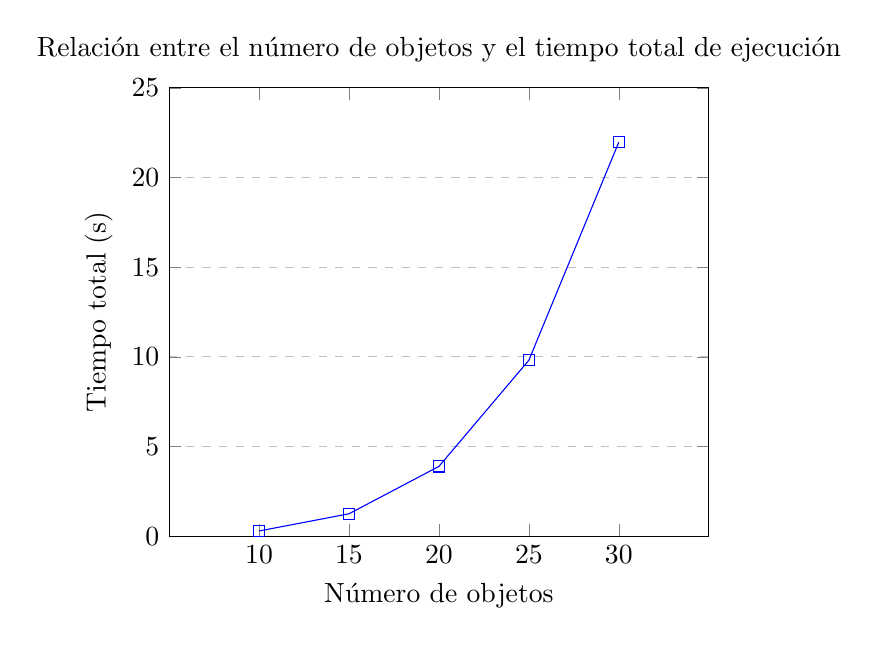
\begin{tikzpicture}
\begin{axis}[
title={Relación entre el número de objetos y el tiempo total de ejecución},
xlabel={Número de objetos},
ylabel={Tiempo total (s)},
xmin=5, xmax=35,
ymin=0, ymax=25,
xtick={10,15,20,25,30},
ytick={0,5,10,15,20,25},
legend pos=north west,
ymajorgrids=true,
grid style=dashed,
]

\addplot[
color=blue,
mark=square,
]
coordinates {
(10,0.29)(15,1.25)(20,3.89)(25,9.81)(30,21.97)
};

\end{axis}
\end{tikzpicture}
\end{center}

\begin{center}
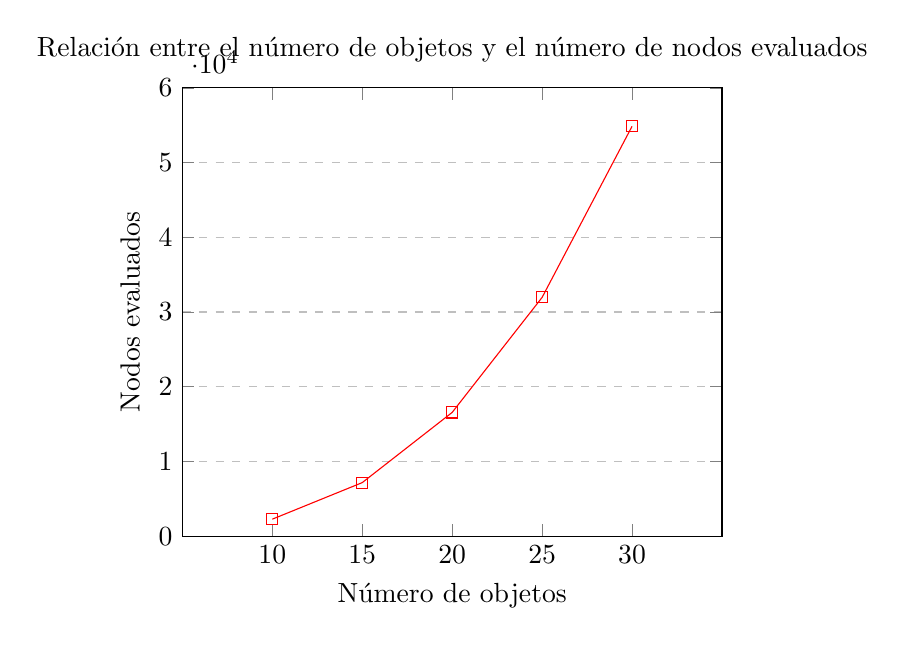
\begin{tikzpicture}
\begin{axis}[
title={Relación entre el número de objetos y el número de nodos evaluados},
xlabel={Número de objetos},
ylabel={Nodos evaluados},
xmin=5, xmax=35,
ymin=0, ymax=60000,
xtick={10,15,20,25,30},
ytick={0,10000,20000,30000,40000,50000,60000},
legend pos=north west,
ymajorgrids=true,
grid style=dashed,
]

\addplot[
color=red,
mark=square,
]
coordinates {
(10,2274)(15,7169)(20,16564)(25,31959)(30,54854)
};

\end{axis}
\end{tikzpicture}
\end{center}

\section{Conclusión}
Este trabajo permitió adentrarse en la complejidad de la planificación automática mediante la manipulación de problemas PDDL y 
el uso del planificador Metric-FF. Si bien se logró resolver la mayoría de los problemas, se evidenció una brecha entre las
 soluciones óptimas y las obtenidas por el planificador.Además, se puso de manifiesto cómo el aumento de la complejidad y/o el número de variables involucradas puede incrementar significativamente el tiempo de ejecución en este tipo de problemas.
\end{document}


